\chapter{Basic principles of RFID}

\section{Contextualization} \label{sec:contextualization}

The concept of identification with the aid of \ac{rf} dates back to the late 1930s. 
The primitive biplanes made of wood and fabric used in Word War I, evolved to all-metal monoplanes by the time of World War II. They were capable of carrying heavy quantities of explosives and travel at hundreds of km per hour, making visual identification of incoming aircrafts obsolete.
This triggered the investment and science in microwave radar.
By the time of the World War II, both fronts were using radar technologies to detect approaching planes. 
Still, remained the problem of identifying allies and enemies planes.
The attack at Pearl Harbor in $1941$ was possible due to a mistaken assignment of incoming Japanese aircraft to an unrelated \ac{us} bomber flight.
The German aircraft force, \emph{Luftwaffe}, found out that as pilots rolled their planes, it would change the radio signal reflected back. This ingeniously simple maneuver became a system that could identify German aircrafts from Allies, being roughly the first \ac{rfid} passive application.~\cite{dobkinRFRFIDSecond2012}

It was soon later, that Watson-Watt, under a British project, developed the first \ac{rfid} active application for \ac{iff} system. An active \ac{rf} transmitter was attached to British planes, which on receiving radar signals from base stations, broadcasted a signal identifying the aircraft has allied.~\cite{HistoryRFIDTechnology}

This established the core concept of today's systems that make this dissertation possible - the over the air identification of transponders~\footnote{a device that, upon receiving a signal, emits a different signal in response}.

The technology kept advancing through the 1950s and 1960s, mainly in the academic field. Companies started to commercialize anti-theft systems based on 1-bit tag~\footnote{a simple inductive RC resonant circuit that detects transponders in field by changes in the reader coil voltage~\cite{andreventuradacruzmarnotozuqueteIdentificacaoPorRFID2018}}.

In the 1970s the first patents were registered on active tag with rewritable memory and a passive transponder for door lockers. The \ac{us} National Laboratory of Los Alamos was asked, by the Energy Department, to developed a tracking system for nuclear materials. The Agricultural Department also requested Los Alamos for a animal tracking system that was design based on \ac{uhfrfid}. These technologies were also transposed by the same engineers to automated toll payment systems in the private market~\cite{landtHistoryRFID2005, HistoryRFIDTechnology,casierAnalogCircuitDesign2011}.

The 1980s experienced the boom of \ac{rfid} development with wager by the private industries and the development of the personal computer.

The 1990s, with the growing and high deployment of the technology, the first standards were developed. 

The 2000s followed the same maturation process but with slow adoption rate in the late part of the decade. 
Despite the interest presented by the retail giants, like Wal-Mart, and investment by the \ac{dod}, the compromises created by the \ac{rfid} industry didn't justified the commitment. The high cost for investment, technical performance difficulties, conflicting standards, security issues and privacy concerns made the investment stale~\cite{RFIDAdoptionStalls}. 
Companies had to strangle \ac{rnd} resources due to inexistent tools and complex implementations, which were required to develop tools for the marketing/sales departments, that truly make use of the \ac{rfid} infrastructure to increase revenue.
Making suppliers adapt to \ac{rfid} also seemed to be a problem, since many companies don't have \ac{rnd} resources at all to begin with~\cite{gaudinSuppliersGainFailed2008}.
Another big issue was the standardization of coding schemes in RF tags. The fight for dominance in the \ac{uhfrfid} market led to multiple coding standards and protocols that made inter-operation among vendor and suppliers infeasible, if not impossible.

In the last decade, despite the advancements in the industry and the adoption by big apparel retailers like Zara, Decathlon and Marks \& Spencer~\cite{RFIDRetailApparel}, there are issues that could inhibit wide-scale use which will be discussed in section~\ref{currentproblems}.

\section{\ac{rfid} System}

\ac{rfid} is an identification technology that uses radio waves or electro-magnetic fields to automatically identify physical objects and collect data about them.
As such, an \ac{rfid} system is a collection of components that implement an \ac{rfid} solution.

The simplest and most elementary \ac{rfid} system starts with a radio device called tag. The tag is attached to the object that needs to be identified. When such a object is presented in front of an antenna connected to a suitable \ac{rfid} reader, the tag transmits this data to the reader via the reader antenna. The reader then forward the information through a communication channel to a software application running on a computer.

Different references describe different specifications of which components comprise an \ac{rfid} system and where they are implemented in concrete terms.
In fact, depending on the use case and requirements, these components can be implemented in different places or not implemented at all.

In the most simplified description, an \ac{rfid} system is usually composed of three physical blocks: \emph{Transponder} that is attached to the physical object and is responsible for storing and transmitting data about it, \emph{Reader} which interact with the transponder to read and write data, and \emph{Software system} that encompass all kinds of hardware and software components that are separated from the reader and support back-end infrastructures and business logic.

From these, all components can be specified and clearly added to one of the blocks.
The prevalent components used in \ac{rfid} systems can be encompassed under one of the following descriptions:

\begin{description}
    \item[Tag] \ac{rf} device that can store and transmit data in a contactless manner using radio waves.
    \item[Reader] also called \emph{interrogator}, is a device that can read from and write data to compatible \ac{rfid} tags.
    \item[Reader Antenna] is a device that is attached to a reader and is responsible for the \ac{rf} interface with the tag.
    \item[Controller] is an interface that allows an external entity to communicate with and control a reader's functions and devices connected to it.
    \item[Sensor, actuator and annunciator] are optional components used for external input and output of the system.
    \item[Host and software system] is an term for all hardware and software components that are separated from the reader device (e.g.\ middleware, back-end infrastructure, point-of-sale terminals, etc.)
    \item[Communication infrastructure] is the wired and wireless network and serial connection infrastructure needed to connect the previously listed components
\end{description}

A run through the specificities of most of the components will be done in the following sections. Will only addressed components that are required or desirable for understanding this dissertation.

\section{\acl{em} Concepts} \label{sec:em}

% Readers Notes:
% - Edgar: no inicio parece que as regions são completamente separadas e só nas boundaries é que se percebe que é uma cena progressiva. Ver se re-radiating é uma cena "valida" ou arranjar uma melhor forma de dizer 

\ac{rfid} technologies use \ac{em} fields or \ac{em} waves to transmit information back and forward between reader and tag.
Designing a well performant system requires a good understanding of \ac{em} concepts.
Reading distance, costs, material properties of tagged object and \ac{rf} environments are a few points where engineers need a good understanding of \ac{em} fields and \ac{em} waves to come up with a good \ac{rfid} solution.

\subsection{\emph{Near-field} and \emph{Far-field}}

An \ac{em} field is the phenomenon produced by moving electric charges. It can be described through Maxwell's equations and mathematical abstracted as a combination of an electric field ($\vec{E}$) and a magnetic field ($\vec{B}$) that interact with each other and their surroundings.
These interactions behavior differently as the distance from the source changes and are usually defined as two main regions: \emph{near-field} and \emph{far-field}.

\subsubsection{Near-field}

\emph{Near-field} manifests from the electric and magnetic fields near the charges and current that directly produced them. It is the region where phenomena like \ac{em} induction and electrostatic occur.
This field can be further split in two regions: reactive \emph{near-field} and radiative \emph{near-field}.

Is in the reactive region that \emph{near-field} \ac{rfid} technologies are defined for. It is the closest to the transmitting antenna and is characterized by non-radiative behaviors. In this region, if the energy is not absorbed by a receiver, self-capacitance and self-inductive effects cause the antenna to store energy very near its surface. When electrons from a nearby conductor are placed in this region, field reactive \emph{near-field} energy is transferred to them, resulting in an energy drain on the transmitter by a change in the impedance viewed by the reader.

In the radiative \emph{near-field}, i.e.\ Fresnel region, the back-coupling of the fields becomes out of phase with the antenna signal, and thus cannot efficiently return inductive or capacitive energy from antenna currents or charges.
In this region conductive objects, such as shelve metal structures, can behave as antennas by inductively receiving and then "re-radiating" some of the energy~\cite{ElectromagneticRadiationField}.

In the context of \ac{rfid} technologies, only the reactive zone is considered when referring to the \emph{near-field} region. The radiative zone is \textit{ineffective} and rather unpredictable and usually not accounted referring to \ac{rfid}.

The power of the field differers between components with the distance ($d$) from the antenna. The magnetic field strength is proportional to $1/d^3$ and the electric to $1/d^2$. The \emph{near-field} components are quite powerful but usually only suited for close range \ac{rfid} technologies due to the rapid fall-off with the distance.

\subsubsection{Far-field}

The \emph{far-field} region is the area where the field behaviors as a \textit{normal} radiating field, composed of \ac{em} waves that propagate outwards - i.e.\ electromagnetic radiation.

\ac{em} waves are created as result of uniform vibrations between an electric field and a magnetic field. In other words, \ac{em} waves are composed of oscillating magnetic and electric fields. A change in one of the field components reflects an equal change of the other and one can not exist independently.
These waves are detached from any feedback from the moving charges that produced it. Means that, after the waves leave the transmitter, they are completely independent of both transmitter and receiver, as opposed to the phenomena in the \emph{near-field} region.

In this region the radiation amplitude decreases $1/d$ as the distance ($d$) from the reader antenna increases, being the best option for \ac{rfid} technologies requiring high reading distances (e.g.\ \ac{uhfrfid}).

\subsubsection{Boundaries}

The boundaries between these regions are characterized by locations where the activity of the associated field components are the strongest. This doesn't mean that the other components aren't present. The transition between regions is progressive.

The \emph{near-field} and \emph{far-field} are roughly delimited by approximately one full wavelength of the \ac{rf} wave emitted from a reader antenna.
This can be more precisely defined taking in account the transmitting antenna characteristics.

For antennas whose size is comparable to wavelength or bigger (used in \ac{uhfrfid}), the borders between regions can be seen in figure~\ref{fig:fieldregionsbigantenna}. The \emph{far-field} boundary can be delimited by the Fraunhofer distance, radial from the antenna. The Fraunhofer distance is described by $2D^2 / \lambda$, where $D$ is the largest dimension of the radiator and $\lambda$ the wavelength~\cite{balanisAntennaTheoryAnalysis2005}.

\begin{figure}[!ht]
    \centering
    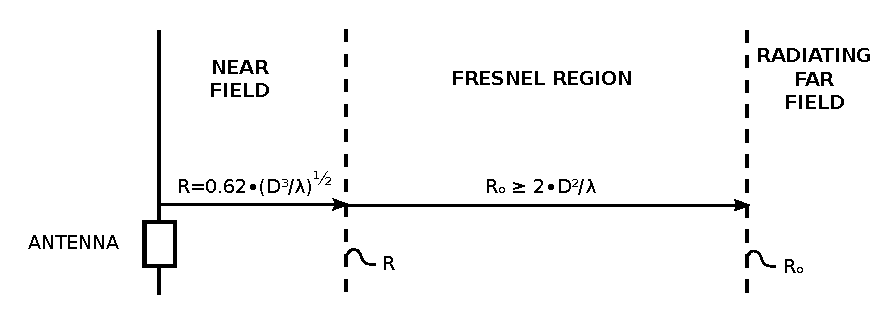
\includegraphics[width=0.9\textwidth]{./figs/02-state-of-the-art/FarNearFields-USP-4998112.pdf}
    \caption{Field for antennas larger than the wavelength of the radiation it emits~\cite{zerodamageFarFieldsVectorized1991}} 
    \label{fig:fieldregionsbigantenna}
\end{figure}

Small antennas, shorter than half of the wavelength of the emitting radiation, (used in \ac{lf}/\ac{hf} \ac{rfid}), the delimitation of fields can be seen in figure~\ref{fig:fieldregionsshortantenna}. The \emph{near-field} for \ac{rfid} applications is usually upper limited by $\lambda / 2\pi = 0.159\lambda$~\cite{nikitinOverviewFieldUHF2007a}. 
For \ac{rfid} technologies that depend upon the \emph{near-field}, these ranges are the physical limit between antenna and transponder.

\begin{figure}[!ht]
    \centering
    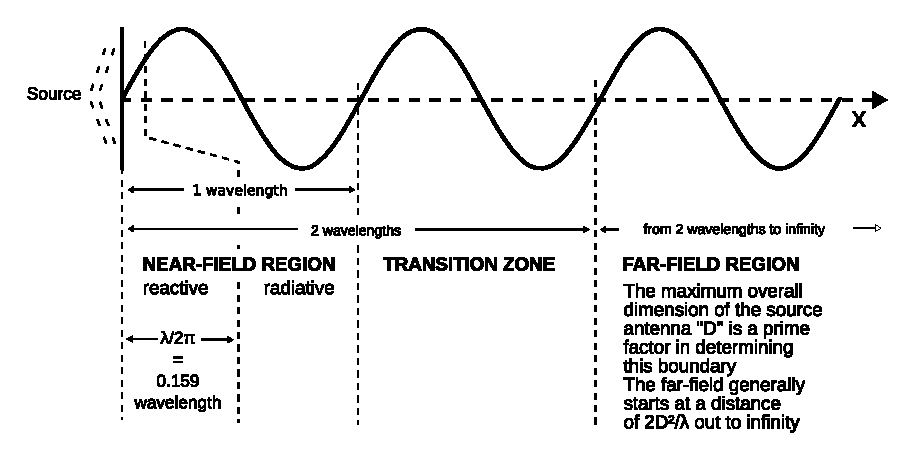
\includegraphics[width=0.9\textwidth]{./figs/02-state-of-the-art/Field_regions_for_typical_antennas_vector.pdf}
    \caption{Fields for antennas equal to, or shorter than, one-half wavelength of the radiation they emit~\cite{SafetyHealthTopics}} 
    \label{fig:fieldregionsshortantenna}
\end{figure}

\section{Tag} \label{sec:tag}

An \ac{rfid} tag is a device that can store and transmit data to a compatible reader in a contactless manner using radio waves of electro-magnetic fields.
It is the center piece of \ac{rfid} systems and essentially what characterizes \ac{rfid} technologies. 

Tag cost is the focus of long term return on investment in \ac{rfid} systems. It is the most important consideration in system design. After the initial investment in infrastructure, the expenses are mainly in the acquirement of tags.
The reduction of cost per tag is the central focus of manufacturers and what allows the technology to be competitive in the world of \ac{scm}.

At its simplest composition, a tag contains a microchip and an antenna.
Depending on the technology the tag architecture and operation varies.
Tags are characterized by their chip, power source, memory characteristics and operating frequency. The following subsections will discussed these in detail.

\begin{figure}[!ht]
    \centering
    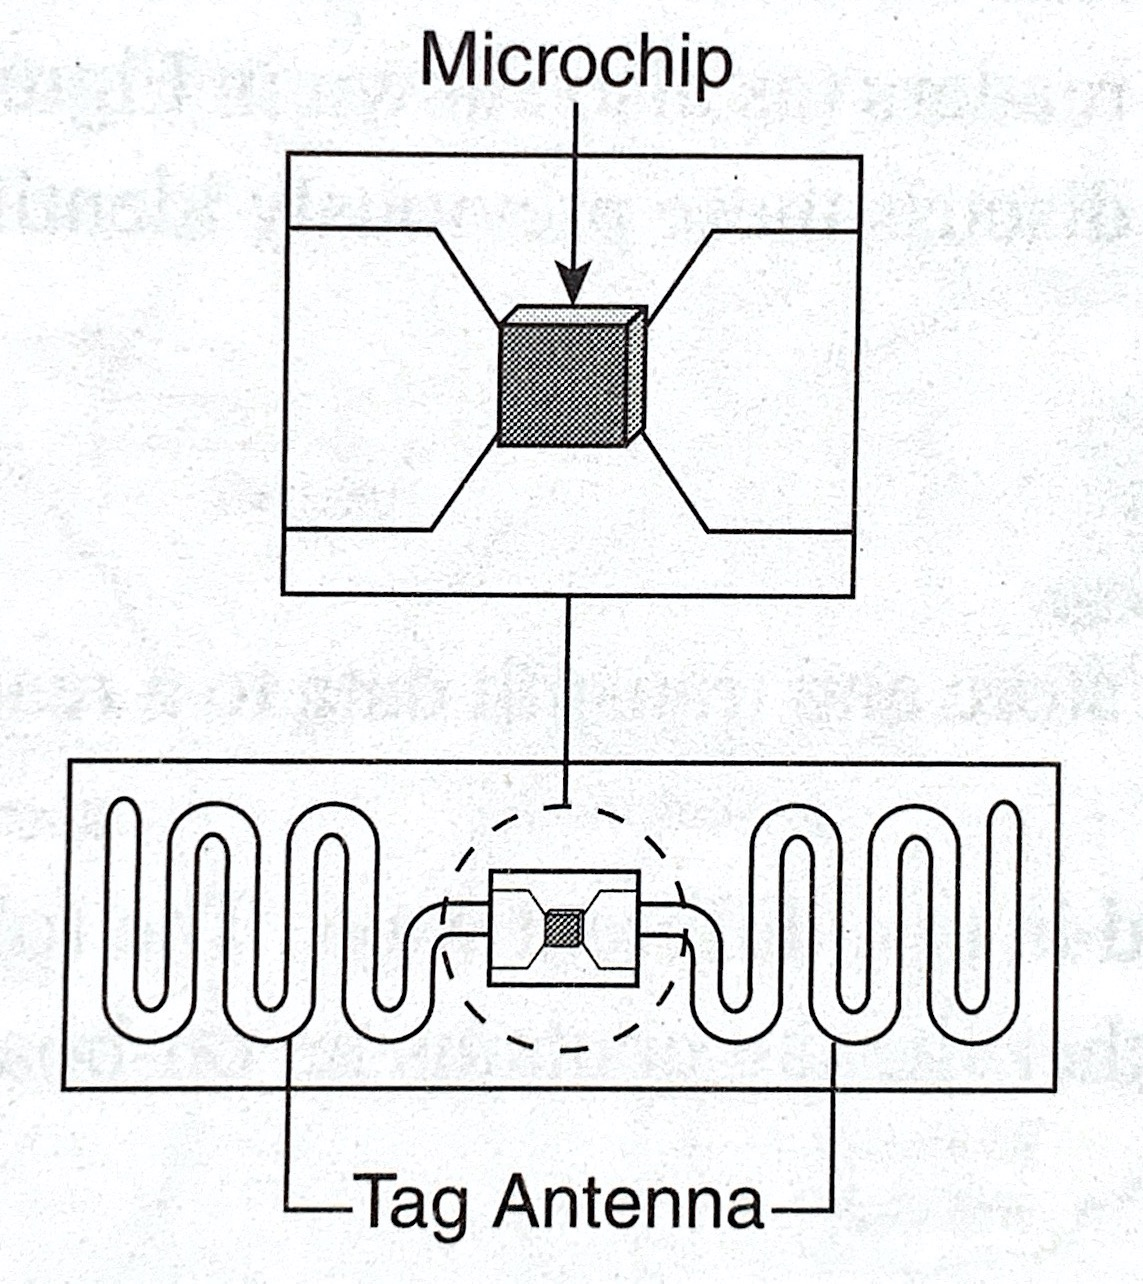
\includegraphics[width=0.2\textwidth]{./figs/02-state-of-the-art/tag.jpg}
    \caption{Components of a passive tag~\cite{lahiriRFIDSourcebook2005}} 
    \label{fig:passivetag}
\end{figure}

\subsection{Data Quantities}

In the contextualization of \ac{rfid} technologies presented in section~\ref{sec:contextualization}, we discussed the concept of identification and how it can be as simple as \ac{iff} systems. 
An unidentified aircraft presents upon radar lightening its identification as being friend or foe. In computing language can be abstracted as true or false, or 1 or 0. This kind of systems does not exchange more than a bit of information, the smallest unit of information that can represent only two states.
This type of transponders are called 1-bit transponders and despite the limitations they are still widely used in surveillance and and anti-theft systems. Apparel retailers and other goods retailers have been using them for almost 6 decades and are still well established nowadays. 
This dissertation requires the identification of more than 2 types of objects, so the following content will jump over technical explanations of this type of transponder. 

The type of transponder discussed through out this dissertation are n-bit transponders which use an electronic microchip as the data carrying device.
These transponders can transfer data in different methods and are currently used in a variety of standards all over the globe.

The following sections of this chapter will approach concepts that are required to understand systems using n-bit tags, specifically \ac{uhfrfid}.
For a deeper analysis of other \ac{rfid} systems you can refer to \emph{The RFID Handbook by Klaus Finkenzeller}~\cite{finkenzellerRFIDHandbookFundamentals2003}.

\subsection{Power Supply}

\subsubsection{Passive}

Passive tags are characterized for not having an on-board power source. 
Instead they use the power emitted from the reader antenna to energize itself and transmit the stored data to the reader.
As such, tag-to-reader communication is always started by a reader, since it needs to energize the tag.

This makes tags simple and cheap to manufacture, a microchip and an antenna is all there is to it.
The simple constitution makes these tags robust, capable of withstanding corrosive chemicals such as acid and high temperatures~\footnote{The new Impinj M730 and M750 \ac{uhf} regular tags for item tagging sustains \ang{206}C for 1 minute and can retain data at \ang{125}C for 1 year~\cite[Tab. 18]{ImpinjM730M750}}.
These are the type of tags that underwent most technology advancements in the last decade in order to meet performance, compatibility and cost expectations that make mass deployment feasible for companies.

\subsubsection{Active}

Active tags have on-board power source and uses it to transmit its data to the reader.
These type of tags don't need the reader's emitted power for data transmission, therefore, in tag-to-reader communication, these tags can either communicate first or be interrogated by a reader.
Usually, active tags stay in a low-power state (i.e.\ sleep) in the absence of interrogation by the reader. When a reader wants to interact with a tag, issues a wake up command. The tag transits out the low-power state and resolves the interrogation.
The \ac{rf} environment generated by systems with these type of tags have much lower \ac{rf} noise, since usually
 they only transmit when interrogated.

Being that the presence of the reader is not necessary for data transmission, an active tag can broadcast its data, like a beacon, to its surrounding even in the absence of a reader. This is what is denominated as \emph{transmitter}.
Widely used for \ac{iot} applications as \textit{wireless computers} to measure, process and transmit information about sensors, but out the scope of this dissertation.

\subsubsection{Semi-passive}

Semi-passive tags, also called \emph{semi-active} or \emph{battery assisted} tag, has on on-board power source but contrary to active tags, is only used for energizing the tag, thus, for transmitting its data, a semi-passive tag uses the reader's emitting power.

There are advantages of using these type of tags over passive ones.
Semi-passive tags do not use the reader signal to excite itself, so it can be read from further distances compared to passive tags. Because no time is needed to energize a semi-passive tag, it can also be read much faster than a passive one, making them useful for applications were the tag is in the reading zone for a short period of time (e.g.\ tolls on highways). Finally, this type of tag might also offer better readability of \ac{rf}-opaque and \ac{rf}-absorbent materials.

\subsection{Coupling}

% Inductive and capacitive coupling (Near-field), Backscatter coupling (Far-field)

We discussed in section~\ref{sec:em} how \acl{em} field behave through the space surrounding the transmitting antenna. Lets now understand how \ac{rfid} technologies take advantage of \acl{rf} to establish a communication interface between reader and tag.

Coupling in \ac{rfid} refers to energy absorbed by a receiving antenna when a transmitting one is operating. 
It is the fundamental concept in passive and semi-passive \ac{rfid} communications.
It affects several aspects of a system including range, frequency and cost.

The method of coupling and the operating frequency are the defining parameters of technology categorization in \ac{rfid}, presented in section~\ref{sec:opfrequency} and used all over the world as a baseline to describe \ac{rfid} systems.

There are three types of coupling techniques: inductive, capacitive and backscatter. These make use of the different field components and radio waves discussed previously.

This dissertation focuses on passive tag systems operating in the remote-couple (i.e.\ range from 1cm to 100cm) and long-range (i.e further than 100cm).
Capacitive coupling is only exploited for capacitive data transmission in close coupling systems (i.e.\ range less than 1cm). Therefore, this type of coupling will not be discussed.

\subsubsection{Inductive}

Inductive-coupling systems, also known as magnetic-coupling, use the \emph{near-field} magnetic component of the \ac{emf} to establish a mutual coupling between reader and tag.

The reader antenna coil generates a strong high frequency \ac{em} field. The variation of the magnetic flux excites the cross-section of the tag coil and induces a voltage.
Because the wavelength of the frequency range used (< 135 kHz: 2400m, 13.58MHz: 22.1m) is several times greater than the distance between reader antenna and the transponder, we can treat it just like a simple inductive coupling system, just like a transformer.

This voltage is rectified and supplied to the tag circuitry.
The circuitry is actually design to resonate at the transmission frequency of the reader. The resonance will generate high current in the reader which produce the required field strength for operation.

To transmit data from tag to reader, inductive systems use load modulation in which the microchip changes de load on its coil in relation with the digital data to transmit. When a transponder, resonant at the transmission frequency of the reader, is placed in the reactive \emph{near-field} region, through mutual coupling, energy is drawn by the transponder, being detected by the reader as a voltage drop in the internal resistance of the reader through supply of current to the reader antenna.

\begin{figure}[!ht]
    \centering
    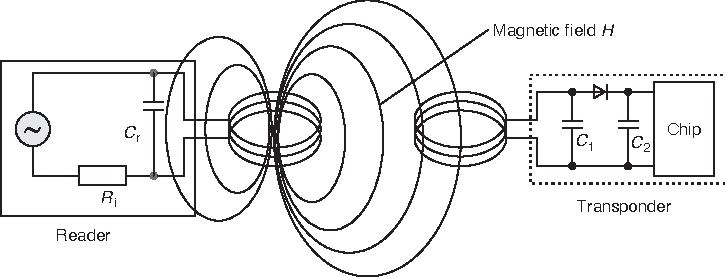
\includegraphics[width=0.9\textwidth]{./figs/02-state-of-the-art/loadmodulation.pdf}
    % Change caption
    \caption{Power supply to an inductively coupled transponder from the energy of the magnetic alternating field generated by the reader~\cite{finkenzellerRFIDHandbookFundamentals2003}} 
    \label{fig:loadmodulation}
\end{figure}

Due to weak coupling between antennas, there are voltage fluctuations at the antenna of the reader, that are much higher than the fluctuations generated by the load modulation in the transceiver. Detecting this slight voltages requires highly complicated circuitry which is undesirable.
Some systems (e.g. 13.58MHz) use what is called load modulation with subcarrier. It uses the side bands created around the operating frequency ($f_T$) for the transmission of data. Switching the load resistor at a high elementary frequency ($f_s$) generates two spectral lines at a distance of $\pm f_s$ which contain the modulated signal. This modulated signal is can them be demodulated by the reader.

\begin{figure}[!ht]
    \centering
    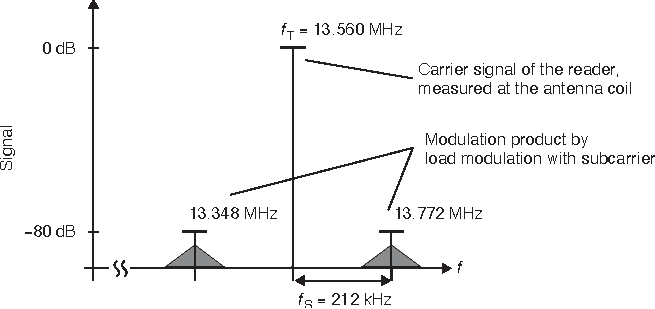
\includegraphics[width=0.7\textwidth]{./figs/02-state-of-the-art/loadmodulation_sidebands.pdf}
    % Change caption
    \caption{Load modulation created two sidebands at a distance of the subcarrier frequency $f_s$ around the transmission frequency of the reader. The actually information is carried in the sidebands of the two subcarrier sidebands, which are themselves created by the modulation of the subcarrier ~\cite{finkenzellerRFIDHandbookFundamentals2003}} 
    \label{fig:loadmodulationsidebands}
\end{figure}

\subsubsection{Backscatter}



\subsection{Technologies} \label{sec:opfrequency}

% absorbent - opaque

\ac{rfid} systems are classified by the frequency band they are used in, which differs between applications:

\begin{table}[]
    \begin{tabular}{|l|l|l|l|l|}
    \hline
    \textbf{Material}     & \textbf{LF} & \textbf{HF} & \textbf{UHF} & \textbf{Microwave} \\ \hline
    Clothing              & RF-lucent   & RF-lucent   & RF-lucent    & RF-lucent          \\ \hline
    Dry wood              & RF-lucent   & RF-lucent   & RF-lucent    & RF-absorbent       \\ \hline
    Graphite              & RF-lucent   & RF-lucent   & RF-opaque    & RF-opaque          \\ \hline
    Liquids (some types)  & RF-lucent   & RF-lucent   & RF-absorbent & RF-absorbent       \\ \hline
    Metals                & RF-lucent   & RF-lucent   & RF-opaque    & RF-opaque          \\ \hline
    Motor oil             & RF-lucent   & RF-lucent   & RF-lucent    & RF-lucent          \\ \hline
    Paper products        & RF-lucent   & RF-lucent   & RF-lucent    & RF-lucent          \\ \hline
    Plastics (some types) & RF-lucent   & RF-lucent   & RF-lucent    & RF-lucent          \\ \hline
    Shampoo               & RF-lucent   & RF-lucent   & RF-absorbent & RF-absorbent       \\ \hline
    Water                 & RF-lucent   & RF-lucent   & RF-absorbent & RF-absorbent       \\ \hline
    Wet wood              & RF-lucent   & RF-lucent   & RF-absorbent & RF-absorbent       \\ \hline
    \end{tabular}
\end{table}

\subsection{Practical considerations}
% Read range depends on, transmitter (reader) power, energy requirements of the tags (for passive tags), absorption factor of materials to which the tag is attached, tag size: the smaller the tag, the smaller the energy capture area, the shorter the read range

% ------------------------------------------------

%The most common classification characteristics are: power - which is based on whether the tag contains on-board power supply and/or harvest energy from the transmitter \ac{rf} waves; and frequency of operation

%Electromagnetic induction if the production of voltage a conductor situated in a changing magnetic flux

%Faraday found that the voltage produced around closed path conductor is proportional to the rate of change of the magnetic flux through any surface

%A antenna of the reader generates a magnetic fields
%The field induces voltage in the coil of the tag and supplies the tag with energy (Faraday's Law)

%Electromagnetic induction if the production of voltage a conductor situated in a changing magnetic flux

%Faraday found that the voltage produced around closed path conductor is proportional to the rate of change of the magnetic flux through any surface



\section{Antennas} \label{sec:antenna}

% Types: circular, linear .. caracteristics of UHF RFID antenna design 

\section{Reader} \label{sec:reader}


\section{Advantages and Limitations}

% --------------------------------------------------------------------------------------------------------------

%Electromagnetic wave propagation is used for data transmission (and powering transponders in the case of passive tags)

%The reader transmits and electromagnetic (EM) wave which propagates outward

%The amount of energy available is decreasing, $1/d^2$, as the distance from the reader increases

%The receiving or transmitting energy is related to the antenna aperture, which related to the wavelength of the sine-wave

%At this frequencies (UHF) we can control the direction of waves, and thus improve the readability in certain areas \dots



%Antennas can also use different polarization for each wave, and this maximize the transmission of information

%The received power can be related to the transmitted power by using the Friis formula that states:

%\begin{equation}
    %P_T = A_{e2} \frac{P_{in}}{4\pi r^2} G_1 = \frac{\lambda^2}{4\pi} G_2 \frac{P_{in}}{4\pi r^2} G_1 \Leftrightarrow P_T = P_{in}  \bigg(\frac{\lambda}{4\pi r} \bigg)^2 G_t G_r
%\end{equation}

\cleardoublepage